\documentclass{article}
\usepackage{mainPoly}

\title{Probabilités conditionnelles}
\author{Terminale STMG2}
\date{}

\begin{document}
\maketitle

\section{Rappels de vocabulaire}
On considère comme exemple d'expérience aléatoire le lancer d'un dé équilibré à 6 faces dont on observe le résultat.
\begin{tcolorbox}
\begin{itemize}
\item L'univers d'une expérience aléatoire, noté $\Omega$, est l'ensemble de toutes les issues possibles $\to \Omega = \{1;2;3;4;5;6\}$ dans le cas du lancer de dé.
\item Un événement est une partie de $\Omega$, c'est ce dont on va évaluer la probabilité $\to$ $A$\og Obtenir un pair\fg est un événement, de probabilité $P(A) = \dfrac{3}{6} = \dfrac{1}{2}$.
\item $\Omega$ est aussi un événement appelé \textbf{événement certain}, avec $P(\Omega) = 1$
\item Si $A$ et $B$ sont deux événements, alors la réalisation de $A$ \textbf{ou bien} de $B$ est modélisée par l'\textbf{union} $A \cup B$ $\to$ l'union de $A$\og Obtenir 2\fg et de $B$\og Obtenir 4\fg est $A \cup B$\og obtenir 2 ou 4\fg.
\item Si $A$ et $B$ sont deux événements, alors la réalisation de $A$ \textbf{et} de $B$ est modélisée par l'\textbf{intersection} $A \cap B$ $\to$ l'intersection de $A$\og Obtenir un pair\fg et de $B$\og Obtenir un $2$ ou un $3$\fg est $A \cap B$\og Obtenir un $2$\fg
\end{itemize}

\end{tcolorbox}

\section{Représentation d'expérience aléatoire}
\begin{example}
Soit une expérience aléatoire d'univers $\Omega$, et deux événements $A$ et $B$ d'$\Omega$. Alors, l'arbre pondéré suivant donne le moyen de calculer certains probabilités.
\begin{center}
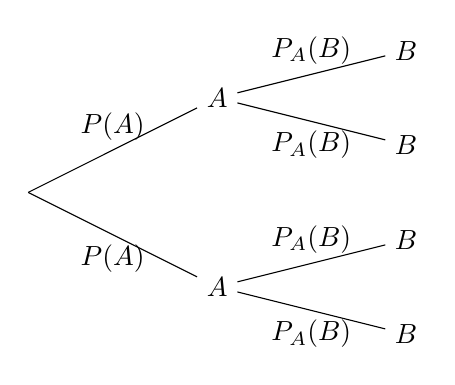
\begin{tikzpicture}[scale=1.2]
\node (A) at (2,1) {$A$};
\node (AB) at (4,1.5) {$B$};
\node (ABn) at (4,0.5) {$\overbar{B}$};
\node (An) at (2,-1) {$\overbar{A}$};
\node (AnB) at (4,-0.5) {$B$};
\node (AnBn) at (4,-1.5) {$\overbar{B}$};
\draw (0,0) -- (A) node[above,midway] {$P(A)$} -- (AB) node[midway,above] {$P_A(B)$};
\draw (A) -- (ABn) node[midway,below] {$P_A(\overbar{B})$};
\draw (0,0) -- (An) node[midway,below] {$P(\overbar{A})$} -- (AnB) node[above,midway] {$P_{\overbar{A}}(B)$};
\draw (An) -- (AnBn) node[below,midway] {$P_{\overbar{A}}(\overbar{B})$};    
\end{tikzpicture}
\end{center}
\end{example}
\begin{tcolorbox}
\begin{proposition}
\hfill
\begin{itemize}
\item Une branche de la racine à une extrémité correspond à l'intersection des événements correspondants. Pour calculer la probabilité de cette intersection, il faut multiplier les probabilités sur la branche.
\item La somme de toutes les probabilités issues d'un même noeud vaut $1$.
\item La probabilité d'un événement est égale à la somme des probabilités de toutes les branches contenant cet événement. 
\end{itemize}        
\end{proposition}
\end{tcolorbox}
\end{document}